\documentclass[12pt]{article}
\usepackage{graphicx}
\usepackage{float}
\usepackage[margin=0.5in]{geometry}

%opening{\normalsize }
\title{{\textbf{Hypothesis}}}
\author{{\textbf{September}}}


\begin{document}
\maketitle
\section{{\large Team Members}}
\begin{center}
	\begin{tabular}{ |c|c| } 
		\hline
		Omnia Zakaria & omniazakaria3112@yahoo.com \\ 
		Reham Hamdy   & rihamhamdy6@gmail.com\\ 
		Zeinab Rabie  & zeinabrabie37@gmail.com\\ 
		Hagar Haytham & hagarhaytham597@gmail.com\\
		\hline
	\end{tabular}
\end{center}
\section{{\large Hypothesis}}
{\textbf {Hypothesis} is a Python library for creating unit tests which are simpler to write and more powerful when run, finding edge cases in your code you wouldn’t have thought to look for. 
Hypothesis lets you write tests which instead look like this:
\begin{enumerate}
	\item For all data matching some specification. 
	\item Perform some operations on the data.  
	\item Assert something about the result.
\end{enumerate}
It generate arbitrary data matching some input specification and checks that some guarantee holds on the output for the generated input, whatever it is. It also saves examples where problems were found to use them for testing again in the future.
 

\section{{\large Getting Started with Hypothesis}}
The main important feature of hypothesis is using strategies for generating different inputs meeting some input specification.
\begin{figure}[H]
	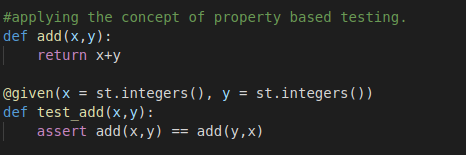
\includegraphics[width=10cm,height=10cm,keepaspectratio]{testing_0.png}
	\caption{Property-based testing.}
	\label{fig 1: Property-based testing.}
\end{figure}
In the previous example, both inputs to the tested functions were generated using hypothesis strategies. Also, there was no assertion on the output value, it only cared about the Add operation having the commutative property.
\begin{figure}[H]
	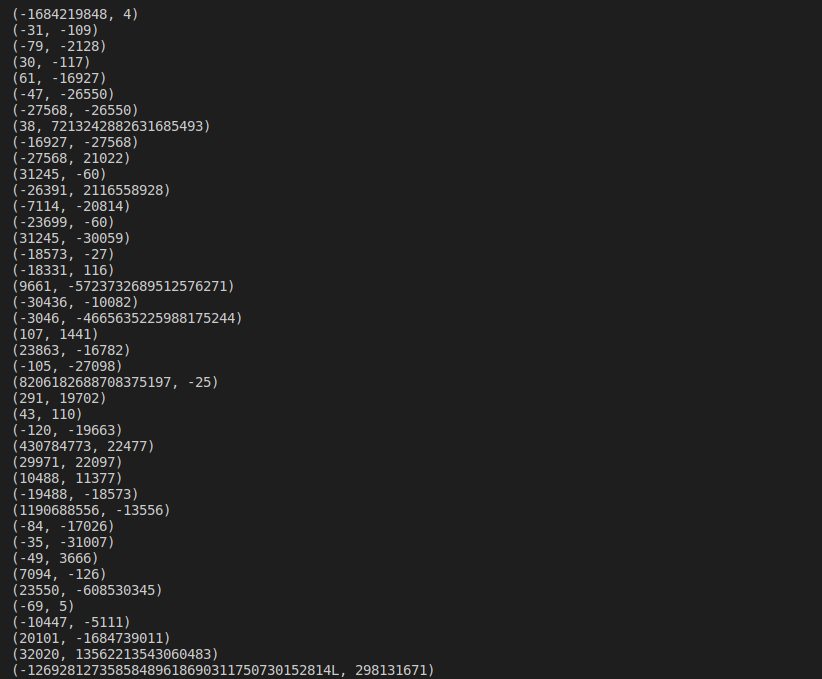
\includegraphics[width=10cm,height=10cm,keepaspectratio]{testing_1.png}
	\caption{A sample of the input generated by strategies.}
	\label{fig 2: strategies' input.}
\end{figure}
And That's basically it to get started with hypothesis, just knowing the correct strategy and the property that's guaranteed in the output of the tested function.
 
\section{{\large Details and Advanced Features}}
This section lists features that are less common in Hypothesis but make life much easier.
Each Feature is followed by a use case.
\subsection{Input Generation: @given}
@given is the entry point of hypothesis to a test function. The @given decorator may be used to specify which arguments of a function should be parameterized over.
\begin{figure}[H]
	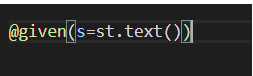
\includegraphics[width=10cm,height=10cm,keepaspectratio]{testing_2.png}
	\caption{Using @given to generate text input.}
	\label{fig 3: Property-based testing.}
\end{figure} 

\subsection{Search Strategies}
The object that is used to explore the examples given to your test function is called a Search Strategy. These are created using the functions exposed in the hypothesis.strategies module. Many of these strategies expose a variety of arguments you can use to customize generation. For example for integers you can specify min and max values of integers to be given to the tested function.
\subsection{Additional test output}
Hypothesis supporting printing out intermediate values during the execution of the test.
 \begin{figure}[H]
 	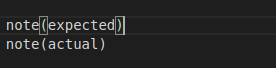
\includegraphics[width=10cm,height=10cm,keepaspectratio]{note.png}
 	\caption{Using note() to print out intermediate values.}
 	\label{fig 3: note.}
 \end{figure}

\subsection{Making Assumptions : assume()}
Sometimes Hypothesis doesn’t give you exactly the right sort of data for the test. You can just ignore these by aborting the test early, but this runs the risk of accidentally testing a lot less than you think you are. Also it would be nice to spend less time on bad examples - if you’re running 100 examples per test (the default) and it turns out 70 of those examples don’t match your needs, that’s a lot of wasted time.
\subsection{Targeted Example Generation : @exmample}
In addition to generating input, Hypothesis also supports specifying some input example that you don't want the test to miss out. 
\subsection{Dependent Strategies : @composite}
One of the important features with strategies is having the ability to generate some strategy based on another. For example: Consider generating some integer then depending on it generate multiple arrays with that integer as their length.
\section{{\large Hypothesis for the Scientific Stack}}
\begin{itemize}
	\item Hypothesis offers a number of strategies for NumPy testing, available in the hypothesis[numpy] extra. It lives in the hypothesis.extra.numpy package. The centerpiece is the arrays() strategy, which generates arrays with any dtype, shape, and contents you can specify or give a strategy for. To make this as useful as possible, strategies are provided to generate array shapes and generate all kinds of fixed-size or compound dtypes.
	\item Hypothesis also provides strategies for several of the core pandas data types: pandas.Index, pandas.Series and pandas.DataFrame 
\end{itemize}.
\section{{\large Limitations}}
\begin{itemize}
	\item Hypothesis mainly focuses on applying the concept of property-based testing. This makes it not able to test different types of software where such concept doesn't apply.
	\item The strategies are not fully customizable. If the software under test required specific inputs, filtering out generated data is not acceptable all time.
	\item To run hypothesis, a strategy have to be specified even if it won't be used. Consider the case when you need a specific input and its corresponding output only. You would still have to specify a strategy even if it's a dummy one and for each input in the strategy, the test will run even if it's doing the same thing.
\end{itemize}
\section{{\large Case Study}}
We used Hypothesis to test A collection of Numerical Analysis functions. For doing that, we used the numpy extension of hypothesis.
\subsection{The Features covered}
\begin{enumerate}
	\item Search strategies : Differrent search strategies were used, adding tweaks to the generated data to match the input specifications of the tested functions.
	\item Targeted Example  : Since the tested functions were made to be custom to some problems, we needed to set some specific input example and make sure that the test passed for these inputs.
	\item Making Assumptions : We made use of this one when manipulating the search strategy wasn't enough. For example: While testing a function that solves a linear system of equations, the coefficients matrix sent to the function should be a non-singular matrix.
	\item Dependent Strategies : Dependent strategies were useful in the case where we needed to test functions on multiple sizes of arrays/matrices. One strategy generated the size and depending on that one, another generated the matrices/arrays.
	\item Disabling health checks : Hypothesis forces a number of examples to be generated in order to guarantee the correctness of the function. in case of limiting the inputs(using assume),the test  
\end{enumerate}
\subsection{Strategies used}
We used strategies for generating arrays, integers, floats, booleans, and also functions based on regular expressions. 
\subsection{Functionalities tested}
\begin{center}
	\begin{tabular}{ |c| } 
		\hline
		Integration \\ 
		Solving Linear systems of Equations \\ 
		Interpolation \\ 
		Ordinary Differential Equations \\
		Partial Differential Equations \\
		Eigen Value Problem \\
		Curve fitting \\
		Extrapolation \\
		
		\hline
	\end{tabular}
\end{center}
\subsection{Limitations}
\begin{enumerate}
	\item Having no ground truth to test the functions on, because the function were implementing approximate methods to solve numerical problems. 
	\item Not being able to exploit the property-based testing offered by hypothesis because the outputs of the functions didn't have a specific property.
	\item Not being able to fully customize the input to meet the input specifications using strategy filtering because it resulted in test health check violations. We had to filter the input ourselves in the test functions. 
\end{enumerate}
\section {{\large Work Load Divison}}
For dividing the work load, each one of us tested some of the Software under test functionalities. 
\begin{center}
	\begin{tabular}{ |c|c| } 
		\hline
		Omnia Zakaria & Solving Linear Systems, RungeODE's, InterpolationDiff, 
		Integration \\ 
		Reham Hamdy   & Eigen Value Problem, PDE's,  Tool Research.  \\ 
		Zeinab Rabie  & Integration, Interpolation, Tool Research.  \\ 
		Hagar Haytham & Curve Fitting,Extrapolation, Tool Research, SUT. \\
		\hline
	\end{tabular}
\end{center}
\section {{\large References}}
\begin{itemize}
	\item Hypothesis Documentation : hypothesis.readthedocs.io.
\end{itemize}

\end{document}
